%%%%%%%%%%%%%%%%%%%%%%%%%%%%%%%%%%%%%%%%%
% Beamer Presentation
% LaTeX Template
% Version 1.0 (10/11/12)
%
% This template has been downloaded from:
% http://www.LaTeXTemplates.com
%
% License:
% CC BY-NC-SA 3.0 (http://creativecommons.org/licenses/by-nc-sa/3.0/)
%
%%%%%%%%%%%%%%%%%%%%%%%%%%%%%%%%%%%%%%%%%

%----------------------------------------------------------------------------------------
%	PACKAGES AND THEMES
%----------------------------------------------------------------------------------------

\documentclass[usenames,dvipsnames,table]{beamer}

\usetheme{Madrid}
%\setbeamertemplate{footline} % To remove the footer line in all slides uncomment this line
%\setbeamertemplate{footline}[page number] % To replace the footer line in all slides with a simple slide count uncomment this line
\setbeamertemplate{navigation symbols}{} % To remove the navigation symbols from the bottom of all slides uncomment this line

\setbeamertemplate{itemize item}[circle]

\usepackage{graphicx} % Allows including images
\usepackage{booktabs} % Allows the use of \toprule, \midrule and \bottomrule in tables
\usepackage{listings}
\usepackage{xcolor}
\usepackage{xfrac}
% \usepackage{enumitem}

%----------------------------------------------------------------------------------------
%	TITLE PAGE
%----------------------------------------------------------------------------------------

\title[ABDA Ch. 7]{Applied Bayesian Data Analysis --- Chapter 7}

\author{Kim Albertsson} % Your name
\institute[LTU and CERN]
{
CERN and Luleå University of Technology \\
\medskip
\textit{kim.albertsson@ltu.se}
}
\date{\today}

\newcommand{\cgy}{\cellcolor{gray!25}}
\newcommand{\cgr}{\cellcolor{green!25}}
\newcommand{\cye}{\cellcolor{orange!25}}
\newcommand{\ccb}{\cellcolor{Cerulean!25}}

\begin{document}

\begin{frame}
\titlepage % Print the title page as the first slide
\end{frame}

%----------------------------------------------------------------------------------------
%	PRESENTATION SLIDES
%----------------------------------------------------------------------------------------
\section{Chapter 7}
\begin{frame}
\begin{center}
{\huge{Chapter 7}}
\\\vspace{2em}
Markov Chain Monte Carlo:\\
Weighted random walks, how to, and their properies.
\end{center}
\end{frame}

\begin{frame}
\frametitle{Personal reflections}
\begin{itemize}
\item The politician island thought experiment felt convoluted. Took some time to understand.
\item Sample representation starts making sense. Still unclear, to me, why the problems of grid based approaches do not apply here.
\item Working through the math here was fun and rewarding.
\item Did not have time to go into details on MCMC accuracy etc. Seems interesting!
\end{itemize}
\end{frame}

\begin{frame}
\frametitle{Today}
\begin{itemize}
\item Unnormalised distributions,
\item Representative Sample, and
\item Two sampling techniques (Metropolis, Gibbs).
\end{itemize}
\end{frame}

\begin{frame}
\frametitle{Introduction}
\begin{itemize}
\item Analytical solution (ch. 6):\\
      Feasible for limited set of prior-likelihood combinations (e.g. conjugate priors).
\item Discretisation on grid (ch. 5):\\
      Curse of dimensionality. (E.g. 6 params with 1000 possibilities each $\to 1000^6 = 10^{18}$ cells in matrix).
\item Representative sample (curr. ch.):\\
      Distribution approximated with samples drawn from distribution.
\end{itemize}
\end{frame}

\begin{frame}
\frametitle{Representative Sample}
\begin{columns}[c]
\column{.4\textwidth}
Representative sample:
\begin{itemize}
\item Assumes: $p(\theta)$, $p(D|\theta)$ calculable up to multiplicative constant.
\item Output: $p(\theta|D)$ as collection of samples to calculate e.g. central tendency and HDI.
\end{itemize}

For intuition: Compare representative sample to polling in politics.
\column{.6\textwidth}
\begin{figure}
\centering
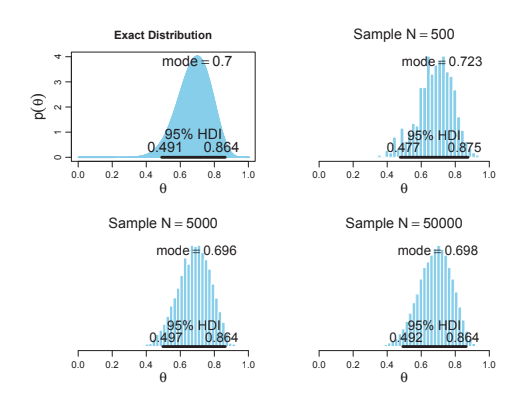
\includegraphics[height=0.6\textheight]{img/fig7_1}
\end{figure}
\end{columns}
\end{frame}

\begin{frame}
\frametitle{A Simple Case of the Metropolis Algorithm (I)}
\begin{columns}[c]
\column{.6\textwidth}
Example: Politician of Island chain
\begin{itemize}
\item Sequential islands
\item Goal: Spend time on island proportional to population
\item Heueristic:
    \begin{align*}
        p_{move} =
            \begin{cases}
            1,                               & \mathrm{if\ } P_{propsed} > P_{current}\\
            \frac{P_{proposed}}{P_{current}},& \mathrm{otherwise}
            \end{cases}
    \end{align*}
\item Metropolis algorithm
\end{itemize}
\column{.4\textwidth}
\begin{figure}
\centering
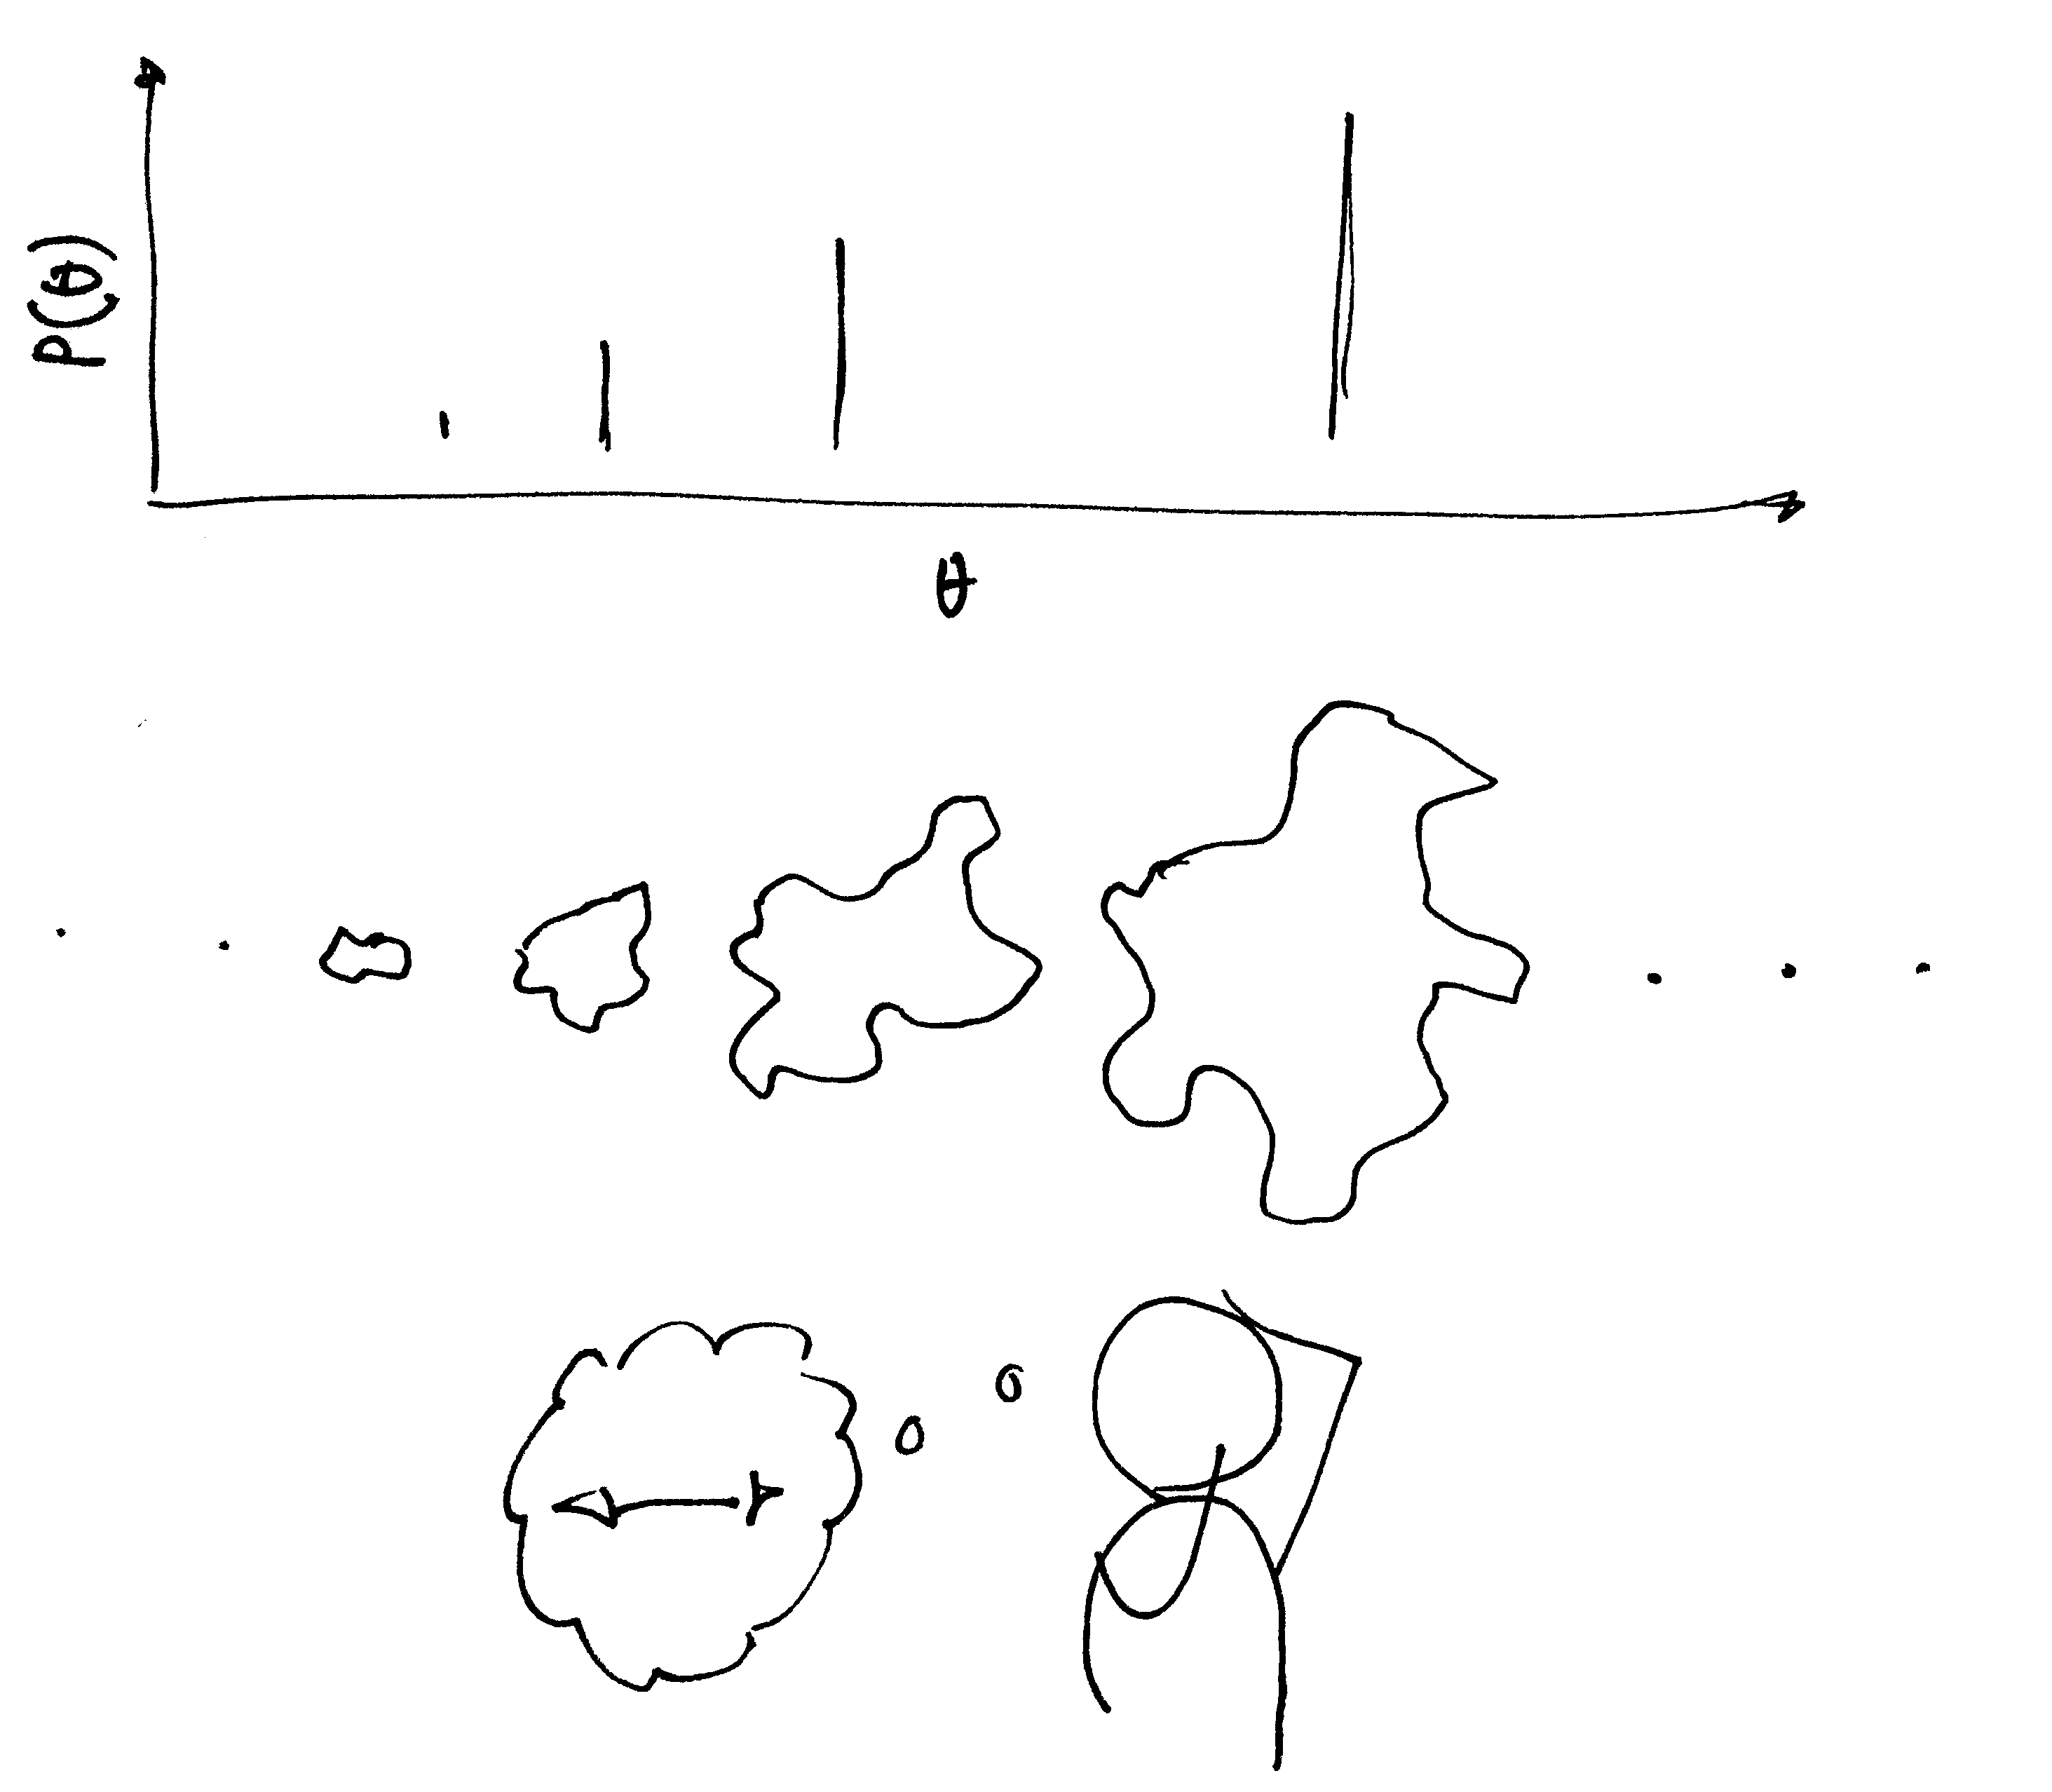
\includegraphics[height=0.4\textheight]{img/experiment-setup}
\end{figure}
\end{columns}
\end{frame}

\begin{frame}
\frametitle{A Simple Case of the Metropolis Algorithm (II)}
\begin{columns}[c]
\column{.5\textwidth}
\begin{itemize}
    \item $P(\cdot)$, relative population. Note: Not normalised!
    \item Top: Relative frequency of visit \emph{after long time}.
    \item Middle: One possible trajectory
    \item Bottom: True distribution
\end{itemize}
\column{.5\textwidth}
\begin{figure}
\centering
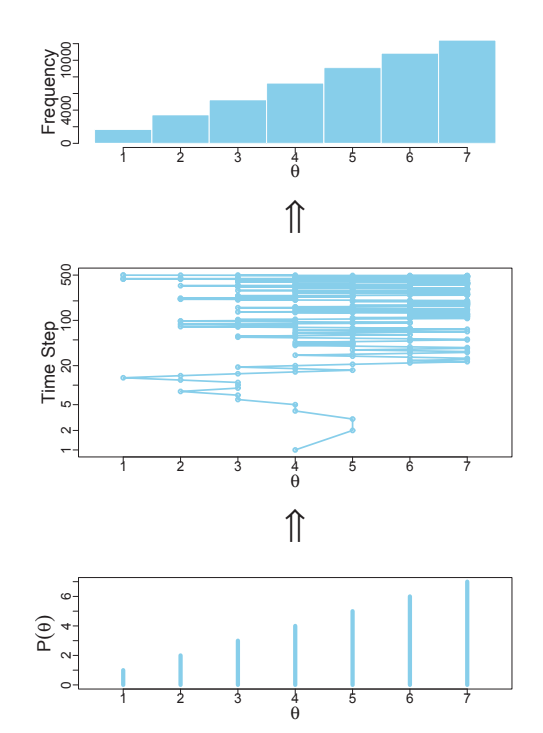
\includegraphics[height=0.8\textheight]{img/fig7_2}
\end{figure}
\end{columns}
\end{frame}

\begin{frame}
\frametitle{A Simple Case of the Metropolis Algorithm (III)}
\begin{columns}[c]
\column{.4\textwidth}
Analysis for this, \emph{simple}, case:

\begin{itemize}
\item Proposal distribution: Moves and probabilities.\\
      Now: $p(\mathrm{left})=0.5$, and $p(\mathrm{right})=0.5$.
\item At time $t=1$ 100\% chance of being in starting position.
\item For $t=2$: \begin{align*}
                    p(\theta=3) =& 0.5 \cdot (\sfrac{P(3)}{P(4)}) \\
                    p(\theta=4) =& 0.5 \cdot (1 - \sfrac{P(3)}{P(4)}) \\
                    p(\theta=5) =& 0.5 \cdot (1)
                 \end{align*}
\item For $t=n$: Iterate...
\end{itemize}
\column{.6\textwidth}
\begin{figure}
\centering
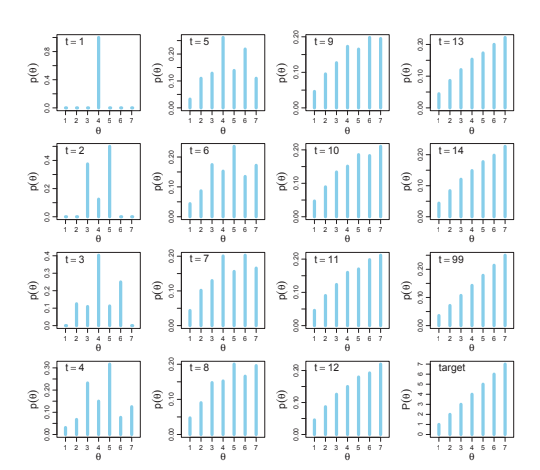
\includegraphics[height=0.6\textheight]{img/fig7_3}
\end{figure}
\end{columns}
\end{frame}

\begin{frame}
\frametitle{A Simple Case of the Metropolis Algorithm (IV)}
\begin{itemize}
\item Uses \emph{proposal distribution}, \emph{acceptance criterion}, and target distribution \emph{ratio}.
\item Convergence to $P(\theta)$ (up to multiplicative constant). 
\end{itemize}

Short form acceptance probability for move:
\begin{align*}
p_{\mathrm{move}} = \min \left(\frac{P(\theta_{\mathrm{proposed}})}{P(\theta_{\mathrm{current}})}, 1\right)
\tag{7.1}
\end{align*}

Intuition for convergence:
\begin{align*}
\frac{p(\theta \to \theta + 1)}{p(\theta + 1 \to \theta)}
    = \frac{0.5 \min{P(\theta+1)/P(\theta)}}
           {0.5 \min{P(\theta)/P(\theta+1)}}
    = \frac{P(\theta + 1)}{P(\theta)}
\tag{7.2}
\end{align*}

Favour travelling to $P(\theta+1)$ more than $P(\theta)$.

(Details: Target distribution is fix point of transition matrix)

\end{frame}

\begin{frame}
\frametitle{The Metropolis Algorithm more generally}
Idea: Random walk through parameter space.
\begin{itemize}
\item Proposal distribution, e.g. $p(M) \mathrm{for} M \in {\mathrm{left}, \mathrm{right}}$, or $p(M) \sim \mathcal{N}$.
\item \emph{Unnormalised} target distribution. Must be calculable for any $\theta$ e.g. $P(\theta) = p(\theta|D)p(\theta)$.
\item Acceptance criterion, e.g. $\sfrac{P(\theta_{t+1})}{P{\theta_{t}}}$
\end{itemize}

\emph{Propose} a move in paramter space. Use \emph{acceptance criterion} to shape distribution of generated samples to match \emph{target distribution}.
\end{frame}

\begin{frame}
\frametitle{Contiuous case (I)}
Example: Estimate bias of coin given some data and prior.
Coin bias: Continuous chain of tiny islands

Note: $P(\theta)$ is tractable b.c. $p(D|\theta)$ and $p(\theta)$ are tractable.

\begin{itemize}
\item Generate jump $\Delta\theta \sim \mathcal{N(o, \sigma)}$. $\theta_{\mathrm{pro}} = \theta_{\mathrm{cur}}+\Delta\theta$.
\item Calculate accpetance $p_{\mathrm{move}} = \min\left(1,
    \frac{\theta_{\mathrm{pro}}^z(1-\theta_{\mathrm{pro}})^{N-z}
          \theta_{\mathrm{pro}}^(a-1)(1-\theta_{\mathrm{pro}})^(b-1) / B(a, b)
         }
         {\theta_{\mathrm{cur}}^z(1-\theta_{\mathrm{cur}})^{N-z}
          \theta_{\mathrm{cur}}^(a-1)(1-\theta_{\mathrm{cur}})^(b-1) / B(a, b)
         }\right)$
\item Accept move if $x \sim \mathcal{U}$ is less than $p_{\mathrm{move}}$, else tally $\theta_{\mathrm{cur}}$ again.
\end{itemize}

Note:
\begin{itemize}
\item More data $\to$ narrower posterior.
\item More samples $\to$ better approximation of posterior.
\end{itemize}
\end{frame}

\begin{frame}
\frametitle{Contiuous case (II)}
\begin{columns}[c]
\column{.4\textwidth}
Example run
\begin{itemize}
\item Left (small steps): High acceptance, inefficient exploration. Low ESS.
\item Mid (medium steps): Medium acceptance, most efficient exploration (of the 3). High ESS.
\item Right (large steps): Low acceptance, inefficient exploration. Low ESS.
\end{itemize}
ESS: Effective sample size
\column{.6\textwidth}
\begin{figure}
\centering
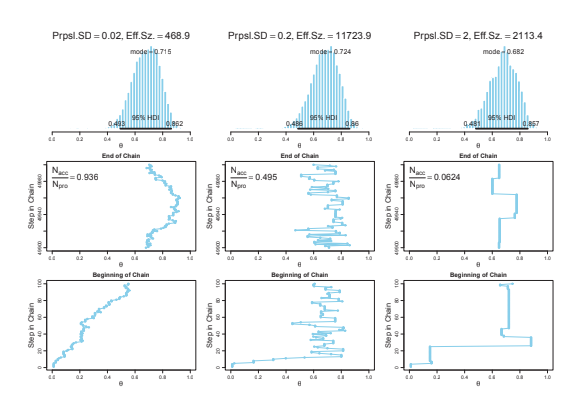
\includegraphics[height=0.5\textheight]{img/fig7_4}
\end{figure}
\end{columns}
\end{frame}

\begin{frame}
\frametitle{Aside: Effective Sample Size}

\textbf{Caveat:} I might have misunderstood this!

\vspace{1em}
Samples in MCMC chain can be correlated.

\vspace{1em}
Effective sample size (ESS) estimates the correlation and reports how many \emph{uncorrelated}, i.e. direct, samples of the target distribution the chain corresponds to.

\vspace{1em}
Source:
\url{http://www.nowozin.net/sebastian/blog/effective-sample-size-in-importance-sampling.html}
\end{frame}

\begin{frame}
\frametitle{Toward Gibbs sampling (I)}
\begin{columns}[c]
\column{.5\textwidth}
Alternative to Metropolis: Gibbs sampling, usually for more than one parameter.

\vspace{1em}
Suppose two coins, each with bias: $\theta = \{\theta_1, \theta_2\}$. Samples from each coin independent.

\begin{align*}
p(\theta)               =& \beta(\theta|a, b)\\
p(D|\theta)             =& \mathrm{Bernoulli}(D|\theta)\\
p(\theta_1, \theta_2|D) =
    &\frac{\theta_1^{z_1+a_1-1}(1-\theta_1)^{N_1-z_1+b_1-1}}
       {B(z_1+a_1, N_1-z_1+b_1)}\\
    &\frac{\theta_2^{z_2+a_2-1}(1-\theta_2)^{N_2-z_2+b_2-1}}
       {B(z_2+a_2, N_2-z_2+b_2)}
\end{align*}

\column{.5\textwidth}
\begin{figure}
\centering
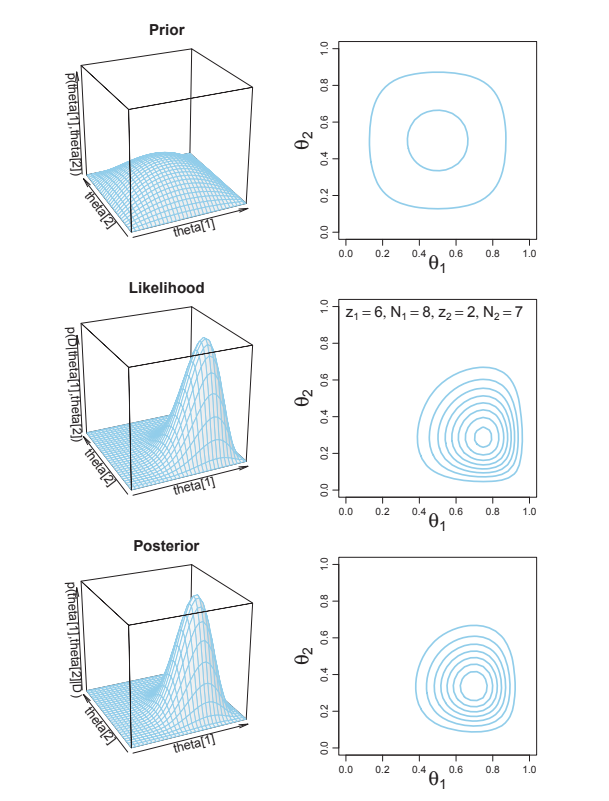
\includegraphics[height=0.8\textheight]{img/fig7_5}
\end{figure}
\end{columns}
\end{frame}

\begin{frame}
\frametitle{Toward Gibbs sampling (II)}
Metropolis estimate of posterior:
\begin{figure}
\centering
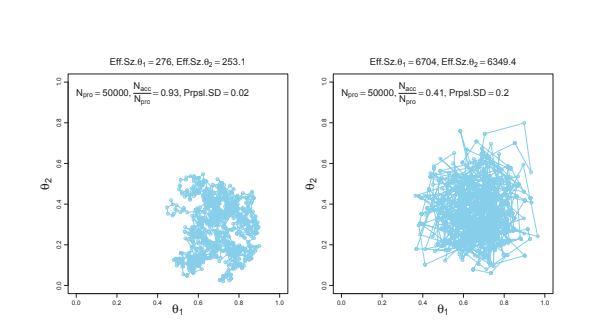
\includegraphics[height=0.7\textheight]{img/fig7_6}
\end{figure}
\end{frame}

\begin{frame}
\frametitle{Gibbs sampling (I)}
\begin{columns}[c]
\column{.6\textwidth}
Idea: Walk only in one paramter direction at a time. Cycle paramters to update.
\begin{itemize}
\item Requires tractable $p(\theta_i|\{\theta_{i\neq j}\}, D)$
\item Cycle paramters ($\theta_1, \theta_2, ..., \theta_1, \theta_2, ..., ...$) to better cover paramter space.
\item Special case of Metropolis: variable proposal distribution
\end{itemize}
\column{.4\textwidth}
\begin{figure}
\centering
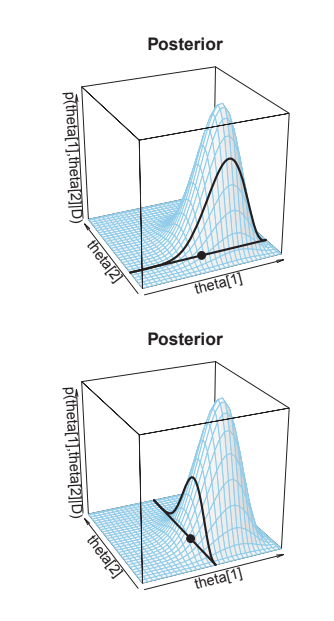
\includegraphics[height=0.8\textheight]{img/fig7_7}
\end{figure}
\end{columns}
\end{frame}

\begin{frame}
\frametitle{Gibbs sampling (II)}
\begin{quote}
Becase the proposal distribution exatcly mirrors the posterior probability for that paramter, the move is always accepted.
\end{quote}
\begin{quote}
Linger at $\theta_1$, building up approximiation of $P(\theta_1, \theta_2)$ for that value. Gibbs sampling does this lingering only one sample at a time.
\end{quote}
\end{frame}

\begin{frame}
\frametitle{Gibbs sampling (III)}
Gibbs sampling estimate of the posterior:
\begin{figure}
\centering
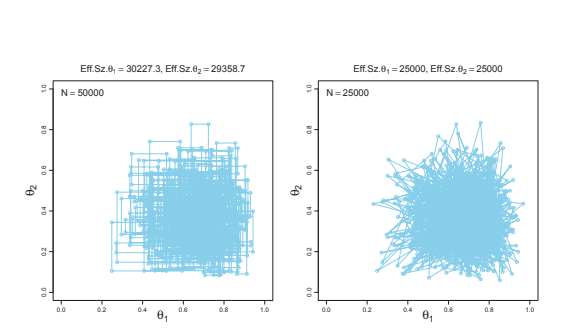
\includegraphics[height=0.7\textheight]{img/fig7_8}
\end{figure}
\end{frame}

\begin{frame}
\frametitle{Representing the posterior}
\begin{columns}[c]
\column{.5\textwidth}
Histogram the representative sample to approximate posterior distribution.

\vspace{1em}
Figure compares results from 4 different generated samples.

\vspace{1em}
Computes estimations of mode and HDI, e.g. for comparing if statistically significant difference.

\vspace{1em}
In limit, all dists should look the same.
\column{.5\textwidth}
\begin{figure}
\centering
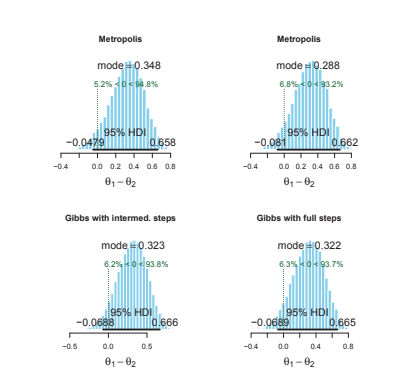
\includegraphics[height=0.6\textheight]{img/fig7_9}
\end{figure}
\end{columns}
\end{frame}

\section{Chapter 7}
\begin{frame}
\begin{center}
{\huge{End!}}
\\\vspace{2em}
\end{center}
\end{frame}

\begin{frame}
\frametitle{Representativeness}
\begin{columns}[c]
\column{.4\textwidth}
Problem: Starting point could be in low-prob area. Algorithm could get stuck in part of the distribution.

\vspace{1em}
Test for convergence (is sample representative): Difficult --- State of the art: Eyeball it.

\vspace{1em}
Burn-in: Up to several thousand samples. Initial samples can be highly non-representative.
\column{.6\textwidth}
\begin{figure}
\centering
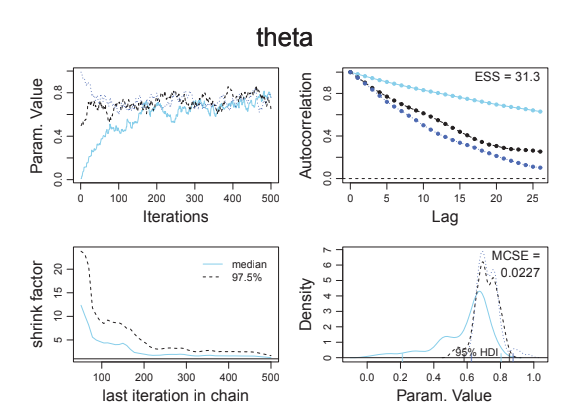
\includegraphics[height=0.6\textheight]{img/fig7_10}
\end{figure}
\end{columns}
\end{frame}

\begin{frame}
\frametitle{Figure 7.11 --- Todo}
\begin{figure}
\centering
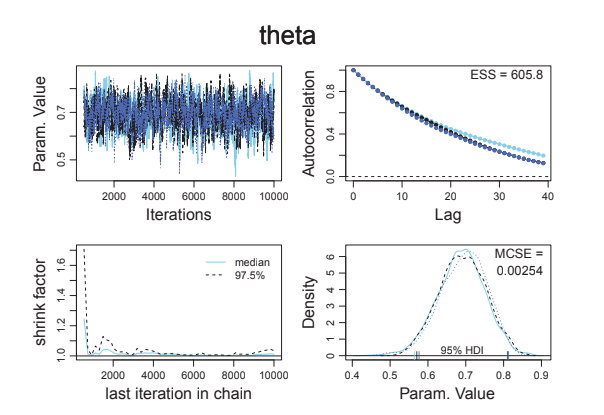
\includegraphics[height=0.8\textheight]{img/fig7_11}
\end{figure}
\end{frame}

\begin{frame}
\frametitle{Figure 7.12 --- Todo}
\begin{figure}
\centering
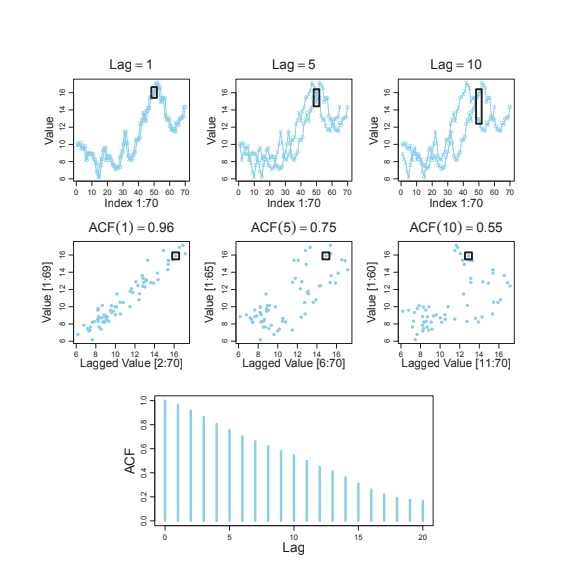
\includegraphics[height=0.8\textheight]{img/fig7_12}
\end{figure}
\end{frame}

\begin{frame}
\frametitle{Figure 7.13 --- Todo}
\begin{figure}
\centering
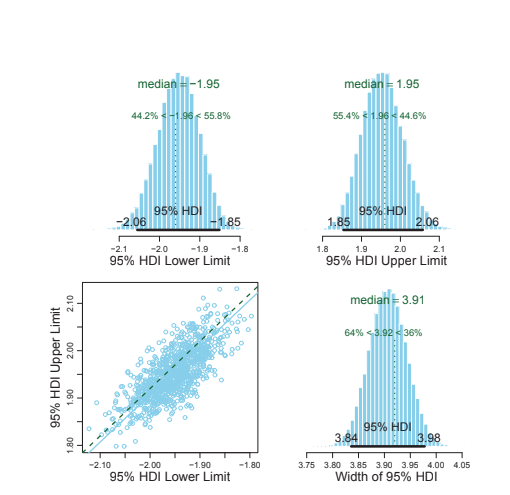
\includegraphics[height=0.8\textheight]{img/fig7_13}
\end{figure}
\end{frame}

\begin{frame}
\frametitle{Figure 7.14 --- Todo}
\begin{figure}
\centering
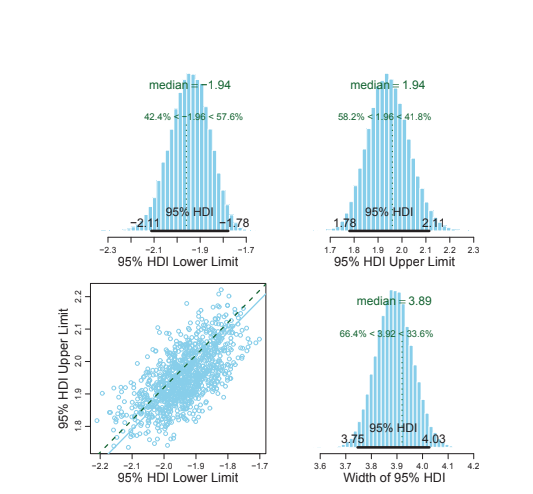
\includegraphics[height=0.8\textheight]{img/fig7_14}
\end{figure}
\end{frame}

% \section{Appendix}
% \begin{frame}
% \begin{center}
% {\huge{For complete code}}
% \\\vspace{2em}
% See \url{https://github.com/ashlaban/ltu-abda-2019/tree/master/ex3}
% \end{center}
% \end{frame}


\end{document} 